\subsection{Prospective Role-Separated Follow-up}
To exercise the protocol's role separation, frozen selection and independent labels, we collected a separate prospective dataset using the same four timer-slack/affinity configurations. The plan was saved before acquisition. Training, retrieval, calibration and test used periods of 2, 3, 4 and $\{5,8\}$\,ms, respectively. Each period had ten randomized four-configuration blocks, with five warm-ups and 40 recorded events per fresh child. This produces 200 measurement processes and 8,000 events. Roles are period-disjoint, not workload-family- or hardware-independent: all runs use the same periodic workload on one shared host. The acquisition manifest validates declared groups, run hashes and graph/calibrator lineage; the analyzer additionally checks freeze timestamps, record completeness and kernel readbacks.

\paragraph{Shared-information non-LLM comparison.}
The empirical selector minimizes mean training-run P95 over the four configurations. A saturated two-factor representation encodes the same four means as a baseline, two main effects and their interaction; minimizing it adds no information to table lookup. Both selectors have the same 40 training runs and zero online search trials. An unchanged-control selector and a seeded uniform-random selector provide references. Choices are frozen before calibration and test. We evaluate these fixed selectors by paired \emph{offline replay} on the same measured test grid, not by separate closed-loop executions. A block is the uncertainty unit, and paired reductions are calculated within each period against its explicit control.

\begin{table}[t]
\centering\small
\caption{Follow-up selector replay: mean of ten test-run P95 values. Misses are observed lateness above 200\,$\mu$s. Shared rows across selectors are intentional: selectors choosing the same configuration use the same held-out observations.}
\label{tab:controlled-selectors}
\begin{tabular}{rlrr}
\toprule
Period & Selector & P95 ($\mu$s) & Misses \\
\midrule
5 & control & 179.7 & 13/400 \\
5 & empirical min & 179.7 & 13/400 \\
5 & graph min & 179.7 & 13/400 \\
5 & seeded random & 811.6 & 248/400 \\
8 & control & 155.7 & 13/400 \\
8 & empirical min & 155.7 & 13/400 \\
8 & graph min & 155.7 & 13/400 \\
8 & seeded random & 642.2 & 225/400 \\
\bottomrule
\end{tabular}

\end{table}

Both informed selectors chose 50\,$\mu$s slack and all CPUs, identical to control; their paired improvement is exactly zero in this replay. Control P95 is $179.7\pm102.0$ and $155.7\pm64.4\,\mu$s at 5 and 8\,ms (95\% Student-$t$ half-width across ten blocks). The training interaction contrast is $-18.6\,\mu$s; the prespecified normalized-contrast bootstrap emitted no edge because its interval included zero. We do not turn a nonsignificant contrast into a dependency rule or a semantic-reasoning gain. Acquisition took 6.54\,s for training, 8.29\,s for retrieval and 10.15\,s for calibration; graph construction and selection took 0.10\,s, included in calibration-phase wall time.

\paragraph{Independent labels and gate misses.}
For this experiment only, the score is a configuration's training deadline-miss fraction, fixed before calibration; it is not the REST reasoner's self-consistency score. A run is labeled unsafe when more than 10\% of its 40 observed events exceed the predeclared 200\,$\mu$s deadline. Thus the label depends on measured timing, independently of a veto or rollback. Every candidate is executed in an isolated owned process, permitting gate replay with observed outcomes for accepted and vetoed candidates. Calibration uses only 4\,ms runs. The three prespecified $\alpha$ values $\{.05,.10,.20\}$ all yield $\tau=.9225$ because the unsafe-score order statistics are tied.

\begin{figure}[t]
\centering
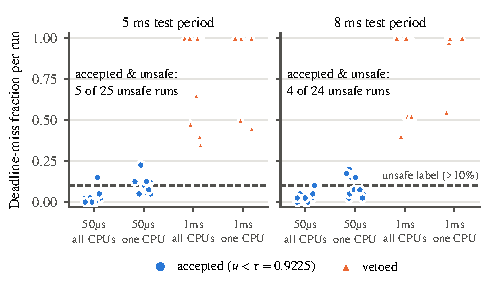
\includegraphics[width=\columnwidth]{figures/gate_replay.pdf}
\caption{Frozen-gate replay on the 80 held-out test runs; each point is one run. Positive means unsafe (dashed line) and a gate-positive decision is veto. Counts at every tested $\alpha$ (all give $\tau=.9225$): 5\,ms, 20 accepted / 20 vetoed, TP~20, FP~0, FN~5, TN~15; 8\,ms, 20 / 20, TP~20, FP~0, FN~4, TN~16. Blue points above the line are the accepted unsafe runs. This is a held-out diagnostic, not prevented production harm. Generated from raw logs by \texttt{plot\_gate\_replay.py}.}
\label{fig:gate-replay}
\end{figure}

Figure~\ref{fig:gate-replay} shows every test run. Unsafe acceptance is $5/25=20.0\%$ and $4/24=16.7\%$ among unsafe runs; unsafe fractions among accepted runs are $5/20=25.0\%$ and $4/20=20.0\%$. Veto precision is $20/20$ in each period, which is not rollback precision. The observed miss rates exceed the nominal 5\% and 10\% levels. Calibration and test periods differ, runs share a host, and the proposition is marginal under exchangeability; these results neither verify its deployment assumptions nor establish recovery. The gate is frozen throughout test, with no retrospective adjustment. The two test periods are different operating conditions, not a drift-recovery trajectory. All counts, thresholds and per-run scores are retained rather than replacing unfavorable outcomes with calibrated claims.

\paragraph{Actual staged application and restoration.}
A separate adapter snapshots the child thread's timer slack and affinity, validates the target, applies both settings, verifies readback, and restores both originals in a \texttt{finally} path, including partial-application failures. These per-thread controls are documented Linux interfaces~\cite{LinuxTimerSlack,LinuxAffinity}. Updates are sequential, not an atomic kernel transaction. The driver observes stages of 8, 16 and 32 events and stops when a stage's deadline-miss fraction exceeds 10\%. Stages are observation counts, not fractions of production traffic. All four configurations are exercised in ten blocks at each test period, independently of the gate replay.

Across 80 fresh executions, 66 stop on a stage breach and 14 complete all stages; all 80 restore and read back both original values. At 5 and 8\,ms, observed deadline misses are respectively $186/816$ and $190/880$; summed exposure durations are 4.106 and 7.066\,s. Early stops reduce the number of observed events, so these fractions cannot be compared directly with fixed-duration, no-stop runs to claim an anomaly reduction. The stop criterion itself is not independent ground truth for rollback precision. The adapter demonstrates bounded actuation and restoration in an owned child; it is not wired into the REST VM-sysctl runtime and does not establish traffic isolation, recovery from irreversible effects or production safety.

\paragraph{Model and explanation audit.}
The audit supplies only frozen training and retrieval evidence and compares full, no-graph, no-retrieval and no-evidence inputs and cited versus matched uncited deletions. Qwen2.5 7B and 14B~\cite{Qwen2024Qwen25}, Llama-3.1-8B~\cite{Grattafiori2024Llama3} and Phi-4 (14B)~\cite{Abdin2024Phi4} ran locally as hashed 4-bit GGUF files in llama.cpp with greedy, schema-constrained decoding. Llama-3.3-70B, Qwen3-235B-A22B~\cite{Yang2025Qwen3}, DeepSeek-V3.2~\cite{DeepSeek2025V32}, Nemotron-3-Ultra-550B~\cite{NVIDIA2026Nemotron3Ultra}, Gemini~3.8 Flash~\cite{Google2026Gemini38Flash} and Gemini~3.1 Pro preview~\cite{Google2026Gemini31Pro} ran through OpenRouter with the same prompts, schema, seeds and temperature~0; they are unhashable and varied across seeds and providers. 249 of 250 calls were valid.

\begin{table}[t]
\centering\footnotesize\setlength{\tabcolsep}{2.5pt}
\caption{Model audit: choice with evidence (full, no graph, no retrieval), without it, and after deletion; superscripts count seeds; n/e: non-estimable; $^\dagger$hosted. Paired test P95 change versus control at 5 and 8\,ms (\%, 95\% half-width): ctrl 0; 50/1 $-145\pm125$ and $-180\pm156$; 1m/all $-599\pm188$ and $-631\pm179$; 1m/1 $-631\pm183$ and $-699\pm206$
\unskip.}
\label{tab:model-audit}
\begin{tabular}{@{}llccc@{}}
\toprule
Model & Context & Choice & 5\,ms & 8\,ms \\
\midrule
Qwen-7B & evidence & 50\,$\mu$s/all & 0 & 0 \\
 & none & 50\,$\mu$s/one & $-145\pm125$ & $-180\pm156$ \\
\addlinespace[2pt]
Llama-8B & all four & 50\,$\mu$s/one & $-145\pm125$ & $-180\pm156$ \\
 & del.\ cited & 1\,ms/all & $-599\pm188$ & $-631\pm179$ \\
 & del.\ unc. & 50\,$\mu$s/all & 0 & 0 \\
\addlinespace[2pt]
Qwen-14B & evidence & 50\,$\mu$s/all & 0 & 0 \\
 & none & 50\,$\mu$s/one & $-145\pm125$ & $-180\pm156$ \\
\addlinespace[2pt]
Phi-4 & evid., del.\ unc. & 50\,$\mu$s/all & 0 & 0 \\
 & none & 1\,ms/one & $-631\pm183$ & $-699\pm206$ \\
 & del.\ cited & 50\,$\mu$s/one & $-145\pm125$ & $-180\pm156$ \\
\bottomrule
\end{tabular}

\end{table}

No model improves on control (Table~\ref{tab:model-audit}). With evidence, all but Llama-8B choose control like the non-LLM selectors; without it, all but Nemotron (a declared default) and one Qwen3 seed choose a worse setting. Faithfulness is non-estimable for models that cite the only table. Deletion changes Llama-8B's choice in both arms and Phi-4's only for cited items, against the remaining runs; for Llama-70B, Qwen3 and Nemotron it changes neither, consistent with the remaining evidence but uninformative about reliance. Of the quantitative claims we checked in explanations, 16 of 28 (local) and 25 of 69 (hosted, full context) are wrong, misattributed, overstated or in the wrong unit. Valid citations establish provenance, not correct reasoning.
